\begin{figure}[h]%
    \centering%
    \begin{subfigure}{.5\textwidth}%
        \centering%
        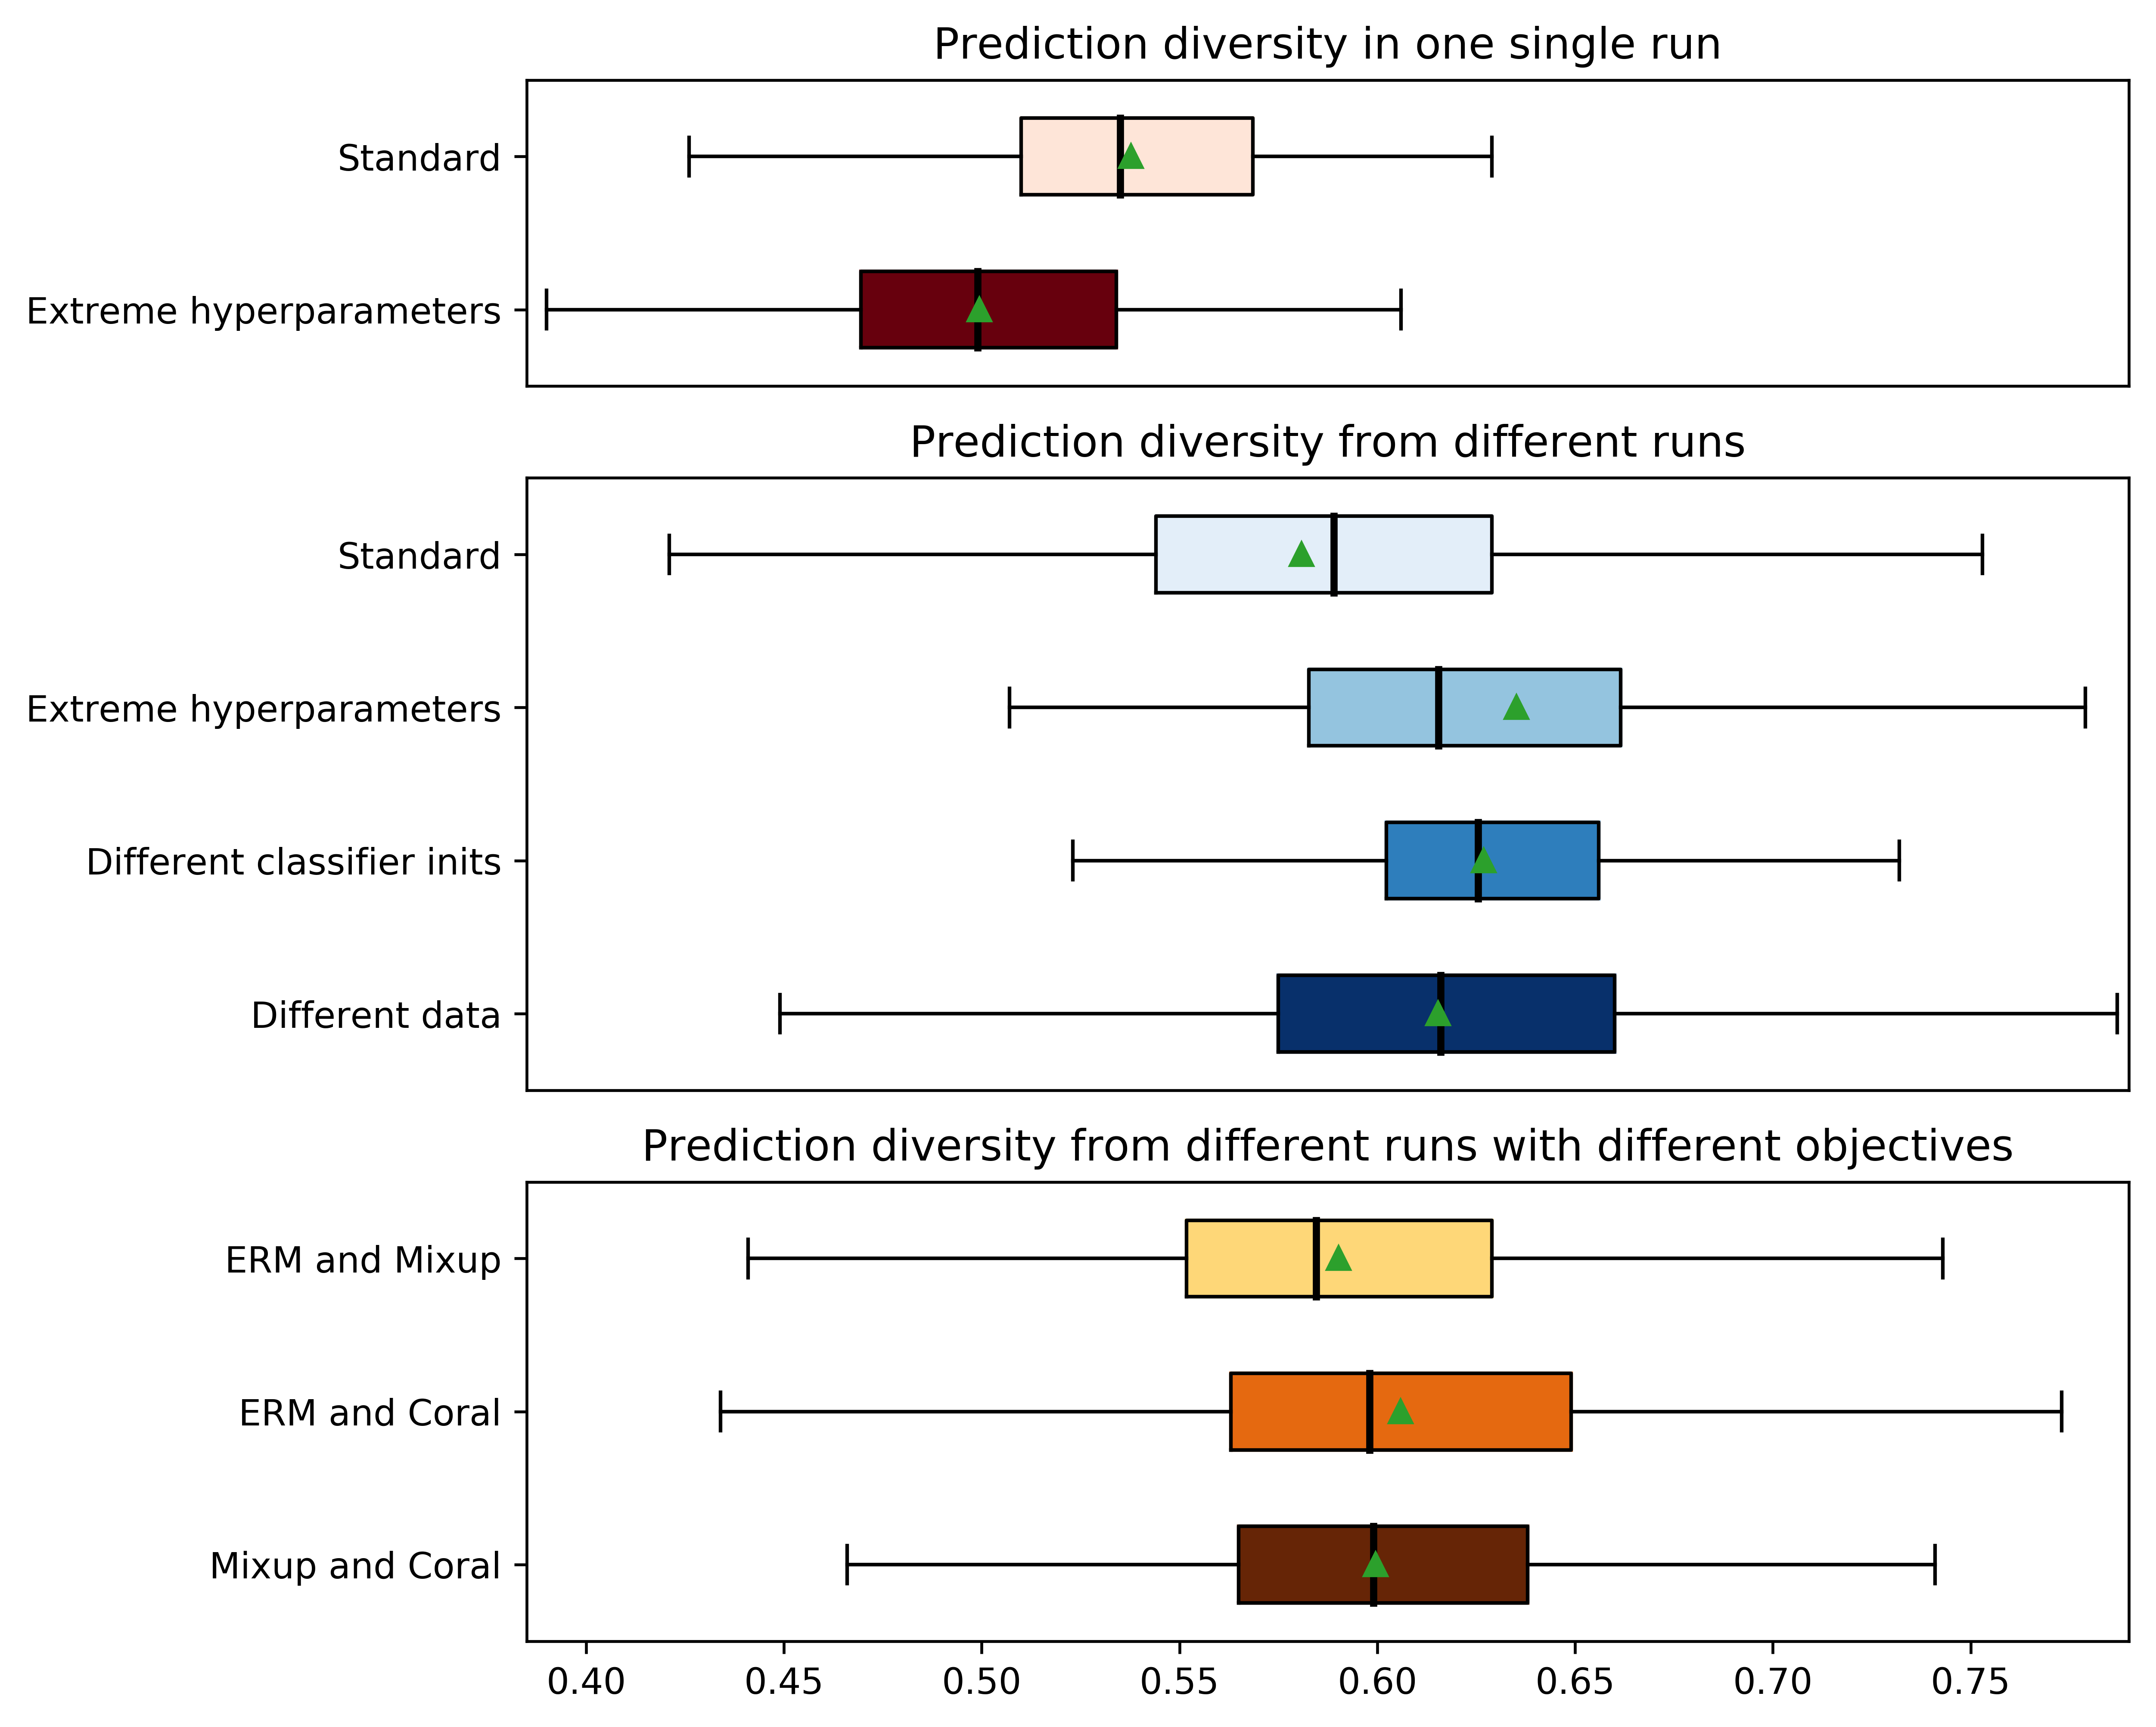
\includegraphics[width=1.0\textwidth]{pictures/files/final/boxplot_dr.png}%
        \caption{Prediction diversity \cite{aksela2003comparison}.}
        \label{fig:home0_dr_boxplot}%
    \end{subfigure}%
    \begin{subfigure}{.5\textwidth}%
        \centering%
        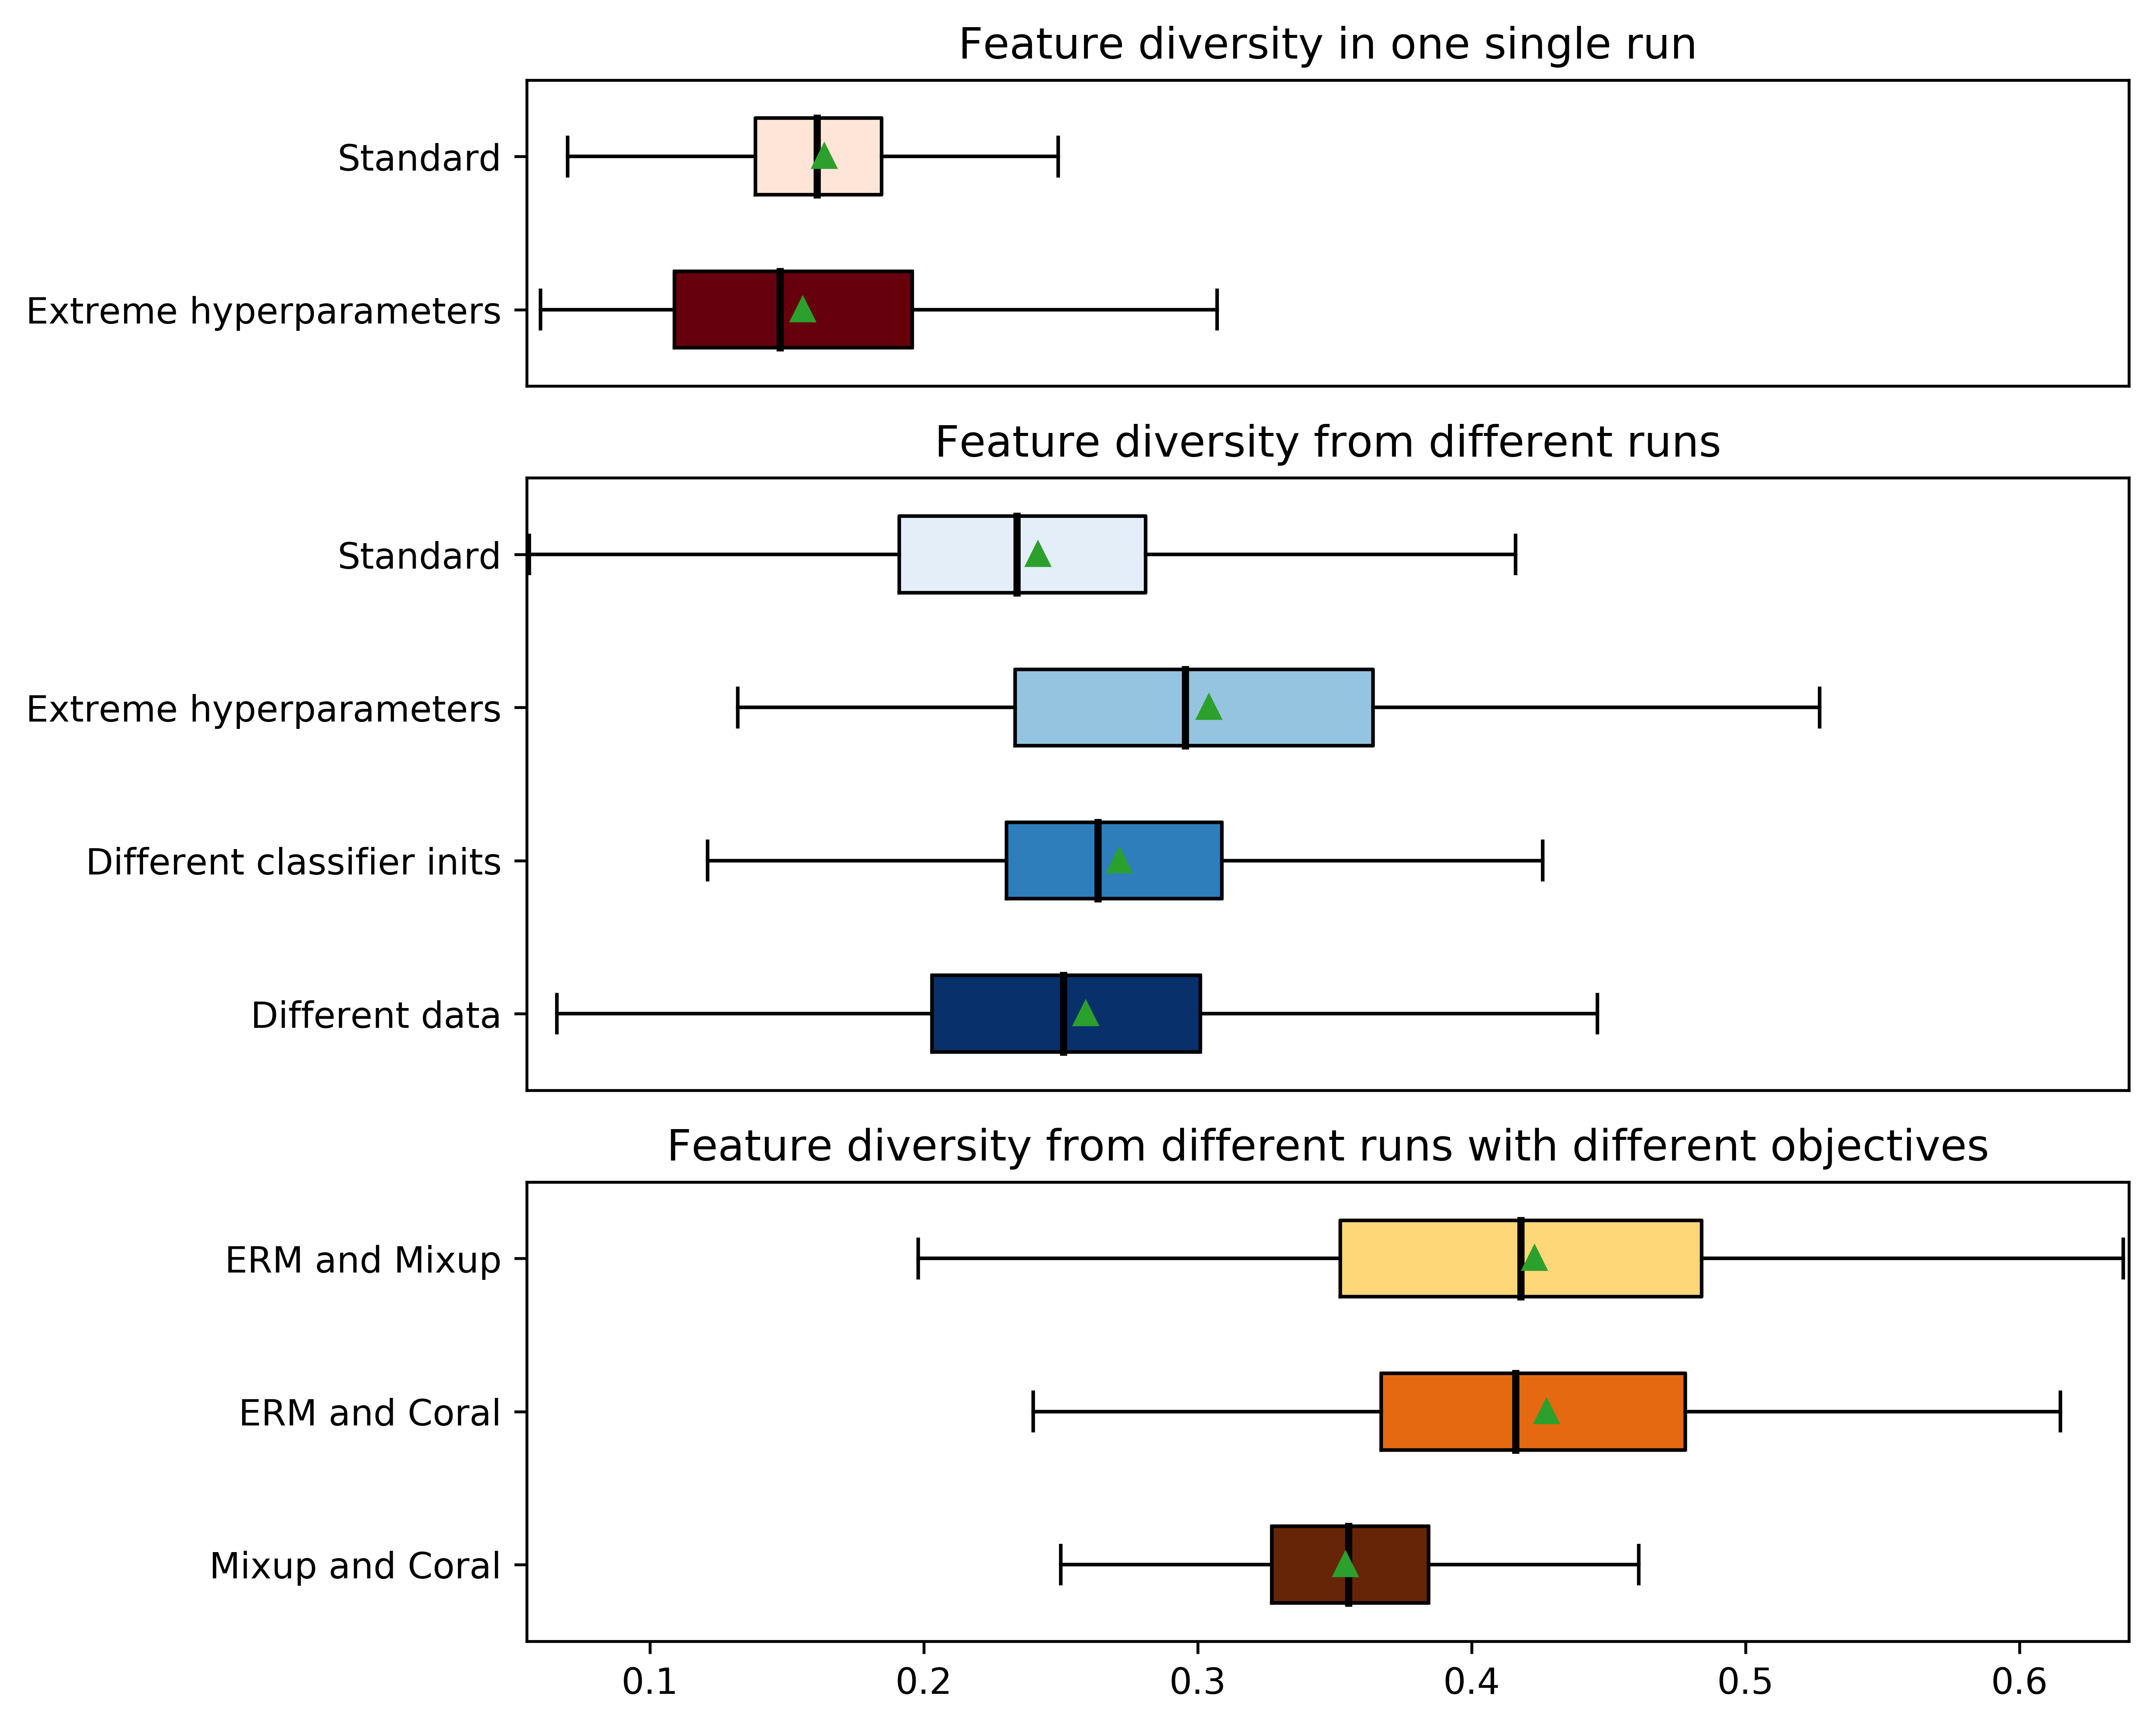
\includegraphics[width=1.0\textwidth]{pictures/files/final/boxplot_df.png}%
        \caption{Feature diversity \cite{DBLP:journals/corr/abs-1905-00414}.}
        \label{fig:home0_df_boxplot}%
    \end{subfigure}%
    \caption{\textbf{Diversity analysis} across weights, which are per default trained with ERM, with a mild hyperparameter range (see \Cref{tab:hyperparam}), with a shared random classifier initialization, on a given data split.
    \textit{First}, it confirms \Cref{fig:home0_dr_frequency,fig:home0_df_frequency}: weights obtained from two different runs are more different than those sampled from a single run (even with extreme hyperparameters).
    \textit{Second}, this shows that weights from two runs are more diverse when the two runs have different hyperparameters/data/classifier initializations/training objectives.
    Domain \enquote{Art} on OfficeHome.}
    \label{fig:home0_boxplot}%
\end{figure}%
